\documentclass{article}
\usepackage[a4paper, total={7in, 9in}]{geometry}
\usepackage[brazil,portuges]{babel}
\usepackage[utf8]{inputenc}
\usepackage[T1]{fontenc}
\usepackage{ebgaramond}
\usepackage{amsmath}
\usepackage{indentfirst}
\usepackage{titlesec}
\usepackage{todonotes}
\usepackage{enumitem}
\usepackage{tikz}
\usepackage{array}
\usepackage{listings}% http://ctan.org/pkg/listings
\lstset{
  basicstyle=\ttfamily,
  mathescape
}
% oi abiguinhos %
\title{Compiladores - Prova 1}
\author{André L. Mendes Fakhoury\\
Gustavo V. V. Silva Soares\\
Eduardo Dias Pennone\\
Matheus S. Populim\\
Thiago Preischadt\\
}
\date{2021}

\begin{document}

\maketitle

\section{Considere a gramática}
\begin{lstlisting}
<S> ::= if <E> then <S> | if <E> then <S> else <S> | acao
<E> ::= a | b
\end{lstlisting}

\subsection{Transforme em uma gramática LL($1$)}

\begin{lstlisting}
<S> ::= if <E> then <S> <S'> | acao
<S'> ::= else <S> | $\lambda$
<E> ::= a|b
\end{lstlisting}




\subsection{Mostre duas árvores de derivação para a sentença "if a then if b then ação else ação"}
eu to com o diagrama no draw.io, ainda vou exportar de novo pra ficar com os níveis da árvore na mesma altura
\begin{figure}[ht!]
    \centering
    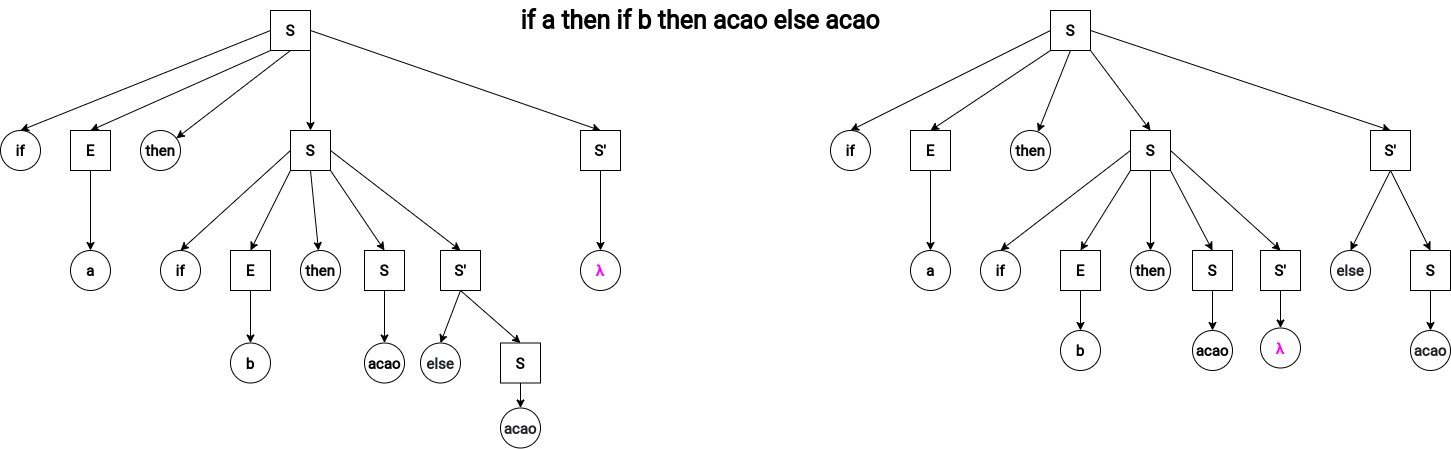
\includegraphics[width=0.9\textwidth]{p1/arvores sintaticas.png}
\end{figure}

\newpage

\subsection{Considerando a ASD preditiva recursiva: crie os grafos sintáticos e implemente os
procedimentos recursivos, incluindo a chamada referente ao símbolo inicial.}

Grafos sintáticos de $\texttt{E,S',S}$. O grafo de $\texttt{S}$ já está no formato reduzido.

\begin{figure}[ht!]
    \centering
    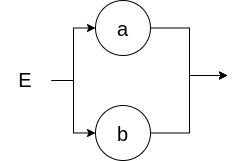
\includegraphics[width=0.2\textwidth]{p1/grafo_sintatico_E.png}
\end{figure}

\begin{figure}[ht!]
    \centering
    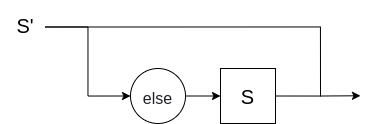
\includegraphics[width=0.4\textwidth]{p1/grafo_sintatico_S_.png}
\end{figure}

\begin{figure}[ht!]
    \centering
    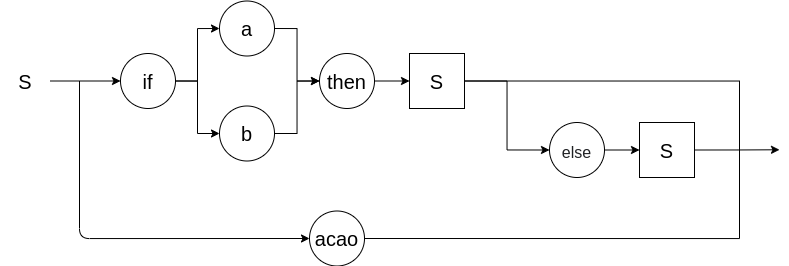
\includegraphics[width=0.9\textwidth]{p1/grafo sintatico.png}
\end{figure}
% kkkkkkkkkkkkkk
% pode mandar?
%https://sites.icmc.usp.br/eugenio/Black_Square.gif <3
% kkkkkkkkkkkkk
%pode sim
% boa noite fakhs, valeu pela paciência!
% boa noiteee, valeuss
 %blacksquare.gif
\begin{lstlisting}
procedimento S'
begin
    se (simbolo = 'else')
        obter simbolo;
        S;
end
\end{lstlisting}


\begin{lstlisting}
procedimento S
begin
    enquanto (simbolo <> 'acao') faca
        se (simbolo = 'if')
            obter_simbolo;
            se (simbolo = 'a') ou (simbolo = 'b')
                obter_simbolo;
                se (simbolo = 'then')
                    obter_simbolo;
                senao erro;
            senao erro;
        senao erro;
        obter_simbolo;
        S';
end
\end{lstlisting}

\begin{lstlisting}
procedimento ASD
begin
    obter simbolo;
    S;
    se terminou_cadeia entao
        sucesso
    senao
        erro
end
\end{lstlisting}


\subsection{Considerando a ASD preditiva não recursiva: crie a tabela sintática. Mostre também uma
inconsistência da tabela. Considerando as linguagens de programação mais atuais, mostre como
essa inconsistência pode ser resolvida.}

\begin{table}[ht!]
\begin{tabular}{|c|c|c|c|c|c|c|c|}
\hline
& \textbf{\$} & \textbf{if} & \textbf{then} & \textbf{acao} & \textbf{else} & \textbf{a} & \textbf{b} \\ \hline
S &  & S ::= if E then S S' &  & S ::= acao &  &  &  \\ \hline
S' & S' ::= $\lambda$ &  &  &  & \begin{tabular}[c]{@{}c@{}}S' ::= else S\\ S' ::= $\lambda$\end{tabular} &  &  \\ \hline
E &  &  &  &  &  & E ::= a & E ::= b \\ \hline
\end{tabular}
\end{table}

A inconsistência ocorre pelo fato das seguintes regras serem ambíguas.
\begin{lstlisting}
S' ::= else S
S' ::= $\lambda$
\end{lstlisting}

Afinal, sabendo que
\begin{lstlisting}
else S = $\lambda$else S
\end{lstlisting}
Vemos a ambiguidade em:

\begin{lstlisting}
S' ::= $\lambda$else S
S' ::= $\lambda$
\end{lstlisting}

Para corrigir isso, podemos aplicar uma regra para diferentes tipos de $\texttt{S}$: um que seja $\texttt{S1}$ e $\texttt{S2}$. S1 é um bloco condicional com $\texttt{else}$, e $\texttt{S2}$ é um bloco condicional sem $\texttt{else}$.
\begin{lstlisting}
<S> ::= <S1> | <S2>
<S1> ::= if <E> then <S1> else <S1> | acao
<S2> ::= if <E> then <S>
<S2> ::= if <E> then <S1> else <S2>
<E> ::= a|b
\end{lstlisting}

A lógica por trás dessa abordagem é garantir que o termo $\texttt{S2}$ nunca seja chamado entre um $\texttt{then}$ e um $\texttt{else}$.

\newpage
\section{Considerando a gramática abaixo, encontre primeiro e seguidor dos símbolos não terminais:}

\begin{center}
\begin{lstlisting}
<E>::=<T><E'>
<E'>::=+<T><E'>|$\lambda$
<T>::=<F><T'>
<T'>::=*<F><T'>|$\lambda$
<F>::=(<E>)|id|$\lambda$
\end{lstlisting}
\end{center}

Neste exercício, o conjunto primeiro de um símbolo $T$ será denotado por $P(T)$, e o conjunto seguidor será denotado por $S(T)$.

Começando pelo conjunto primeiro, é fácil de ver que $P(E') = \{+, \lambda\}, P(T') = \{*, \lambda\}$ e que $P(F) = \{(, id, \lambda\}$.

Calculando agora $P(T)$. Como $\lambda \in P(F)$ e $\lambda \in P(T')$:

$$P(T) = P(F) \cup P(T') \cup \lambda = \{(, id, *, \lambda\}$$

\noindent e, por fim, $P(E)$. Temos que $\lambda \in P(T)$ e $\lambda \in P(E')$, logo:

$$P(E) = P(T) \cup P(E') \cup \lambda = \{+, *, (, id, \lambda\}$$

Portanto, temos os conjuntos primeiros:

\begin{align*}
	P(E) &= \{+, *, (, id, \lambda\}\\
	P(E') &= \{+, \lambda           \}\\
	P(T) &= \{   (, id, *, \lambda                    \}\\
	P(T') &= \{  *, \lambda               \}\\
	P(F) &= \{ (, id, \lambda          \}
\end{align*}	
	
Calculando agora o conjunto seguidor, podemos analisar cada regra de transição.

Começando pela símbolo inicial, temos que $S(E)$ terá $\lambda$ (por ser inicial), e também $)$ por conta da transição $F \rightarrow (E)$. Assim, $S(E) = \{), \lambda\}$.

Pela primeira regra, temos que $S(E') = S(E)$, logo $S(E') = \{), \lambda\}$.

Calculando agora $S(T)$, ele será a união de $P(E')$, por conta de $E \rightarrow TE'$, $S(E)$, por conta de $E \rightarrow TE'$ e $S(E')$, por conta de $E' \rightarrow +TE'$, e $\lambda \in P(E')$. Assim, $S(T) = \{+, ), \lambda\}$.

O $S(T')$ será igual ao seguidor de $T$ (pois $T \rightarrow FT'$), logo $S(T') = \{+, ), \lambda\}$.

E, por fim, temos que analisar todas as regras de transição que possuem $F$ para calcular $S(F)$. O símbolo $\lambda$ está presente em todos os conjuntos primeiro (em específico, no de $T'$ também), e, a partir das transições $T \rightarrow FT', T' \rightarrow *FT'$, temos que $S(F) = P(T') \cup S(T) \cup S(T') = \{*,+,),\lambda\}$.
	
Portanto, temos:

\begin{align*}
	S(E) &= \{ ), \lambda            \}\\
	S(E') &= \{  ), \lambda       \}\\
	S(T) &= \{ +, ), \lambda     \}\\
	S(T') &= \{   +, ), \lambda                    \}\\
	S(F) &= \{ +, *, ), \lambda      \}
\end{align*}

\newpage
\section{Considere as seguintes questões:}

\subsection{Explique a razão pela qual as linguagens de programação são implementadas como linguagens
livres de contexto, embora as informações de contexto sejam importantes, por exemplo, para
identificar se uma variável já foi declarada.}

A maioria das implementações da parte sintática de linguagens de programação são implementadas com gramáticas livres de contexto, portanto a análise sintática é feita através de gramáticas livres de contexto. Mas há um problema: o contexto é importante dentro da linguagem de programação. Quanto mais complexa a linguagem mais difícil tratá-la, isto é, mais difícil desenvolver um método de parser para reconhecer aquela linguagem. No entanto é interessante que a capacidade da gramática não seja muito limitada. A linguagem livre de contexto é suficientemente simples e capaz de gerar toda a complexidade necessária para linguagens de programação, sendo mais complexa do que a linguagem regular, e mais fácil de tratar do que uma linguagem sensível ao contexto. 
% \\

% Existe uma hierarquia definida por Chomsky e refinada por outros pesquisadores acerca de estrutura de linguagens denotadas por sequências de símbolos, palavras, letras, etc. Essa estrutura contém os seguintes níveis:

% 1.	Linguagens finitas.

% 2.	Linguagens regulares - aquelas das expressões regulares.

% 3.	Linguagens livres de contexto - vou explicar abaixo.

% 4.	Linguagens sensíveis ao contexto.

% 5.	Linguagens recursivas (também denominadas decidíveis).

% 6.	Linguagens recursivamente enumeráveis (também denominadas semi-decidíveis).

% 7.	Linguagens irrestritas - ou seja, esta é a categoria mais geral que engloba todas e quaisquer linguagens.
% \\

% Cada nível é um superconjunto do nível anterior. Assim sendo:

% •	As linguagens livres de contexto são mais poderosas e mais gerais do que as linguagens regulares. Ou seja, com linguagens livres de contexto você pode expressar estruturas/linguagens que não podem ser representadas por expressões regulares.

% •	Todas as linguagens que podem ser expressas por meio de uma expressão regular também podem ser expressas por meio de uma linguagem livre de contexto.

% •	As linguagens livres de contexto ainda estão bem longe de serem linguagens capazes de expressar qualquer coisa. Existem alguns níveis acima delas.
% \\

% A hierarquia fica assim:

% \begin{figure}[ht!]
%     \centering
%     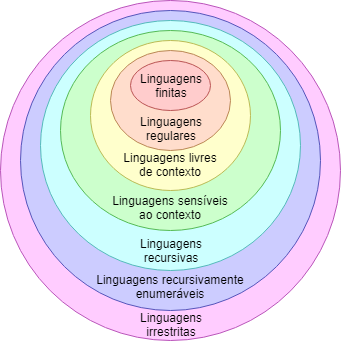
\includegraphics[width=0.4\textwidth]{p1/hierarquia_chomsky.png}
%     \caption{Hierarquia de Chomsky (e refinada por outros pesquisadores). Fonte: <https://pt.stackoverflow.com/questions/180927/o-que-\%C3\%A9-uma-linguagem-livre-de-contexto>}
% \end{figure}

Para realizar a análise semântica seria necessária uma gramática sensível ao contexto, pois tudo o que depende do contexto está relacionado à semântica. No entanto a parte semântica não é tratada através de gramáticas, sendo tratada de maneira informal através de tabelas de símbolos e com anotações semânticas que são feitas na fase de análise sintática. A partir da gramática livre de contexto e feito um parser para que a análise sintática seja realizada, e a ausência de informação de contexto da análise sintática é tratada através da adição de uma nova fase: a fase de análise semântica. Em resumo: Na análise sintática é definida a linguagem de programação através de uma gramática livre de contexto e o tratamento semântico é feito posteriormente, na fase de análise semântica, de maneira informal, com tabela de símbolos e com anotações nas estruturas obtidas na fase de análise sintática. As etapas de análise serão explicadas com mais detalhes na próxima questão.

\subsection{Desenhe a estrutura tradicional de um compilador, incluindo todas as suas etapas e estruturas
de dados auxiliares. Explique a função de cada etapa e estrutura referente à parte de análise.}

\begin{figure}[ht!]
    \centering
    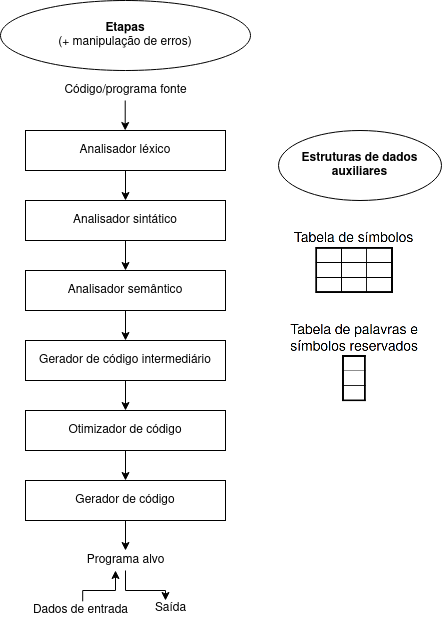
\includegraphics[width=0.43\textwidth]{p1/etapas.png}
    \caption{Estrutura de um compilador. Fonte: baseado nos materiais de aula do Prof. Amancio}
\end{figure}

\textbf{Análise Léxica}
\\

A análise léxica é a primeira fase do processo de compilação e tem como objetivo identificar unidades léxicas ou lexemas que compõem o programa. O analisador léxico lê todos os caracteres do programa fonte, verifica se eles pertencem ao alfabeto da linguagem e, caso um caractere não pertença, é gerado um erro léxico.

Os comentários e espaços em branco são ignorados e removidos e nesse processo um conjunto de \textit{tokens} - que são formados por palavras reservadas, identificadores, delimitadores etc - é formado. Nessa etapa é criada a tabela de símbolos.

Em resumo: a análise léxica quebra o texto do programa fonte em lexemas, verifica a categoria ao qual eles pertencem e produz uma sequência de símbolos léxicos chamados de \textit{tokens}.

O analisador léxico deve permitir identificar na linguagem repetições de subconjuntos permitindo que seja possível identificar e classificar esses subconjuntos, por exemplo o subconjunto de palavras reservadas.

Nessa fase o processamento de uma linguagem pode ser feito por gramáticas regulares podendo ser formalmente descrito por expressões regulares. As rotinas que processam essa linguagem modelam algoritmos construídos a partir de autômatos finitos.
\\

\textbf{Análise Sintática}
\\

A etapa de análise sintática tem como objetivo validar a gramática do programa ao reconhecer se a estrutura gramatical do código fonte está de acordo com as regras sintáticas da linguagem.

Nessa etapa é produzida uma estrutura de dados em formato de árvore conhecida como árvore sintática. Elá é formada após feita uma varredura na sequência de \textit{tokens} recebidas do analisador léxico. A árvore sintática representa a hierarquia do programa fonte. Caso uma construção seja reconhecida com inválida um erro sintético deve ser gerado.

Mesmo com uma boa técnica de detecção de erros o analisador sintático deve ser capaz de recuperá-los e continuar o processo de compilação identificando o maior número possível.

A sintaxe da maioria das linguagens de programação é especificada usando gramáticas livres de contexto que permitem realizar substituições impostas por regras produção e assim validar a estrutura do programa.
\\

\textbf{Análise Semântica}
\\

Essa etapa tem como objetivo verificar se a semântica do programa fonte tem consistência. Para isso é utilizada a árvore sintática e as informações contidas na tabela de símbolos.

A verificação de tipo em uma operação de soma onde cada operando é verificado com cada operador, por exemplo.

Pode ser necessário que nessa fase alguns tipos de dados sejam convertidos para outros tipos, essa operação é conhecida como coerção.
\\

Alguns tipos de erros semânticos:

•	Tipos de operandos incompatíveis com operadores;

•	Identificadores, variáveis e procedimento, não declarados;

•	Chamada de funções ou métodos com número incorreto de operadores;

•	Comandos fora de contextos, um comando continue fora de um laço;

•	Operações de conversão de tipos.
\\

A tabela de símbolos é muito importante nessa etapa pois é através dela que é possível recuperar informações sobre os identificadores que são utilizadas para avaliar as regras semânticas.
\\

\textbf{Tabela de Símbolos}
\\

É utilizada principalmente dentro da fase de análise semântica. Essa tabela é responsável por armazenar os atributos semânticos relacionados às variáveis ou outros elementos importantes dentro do programa. Por exemplo podemos ter uma variável, com a informação de seu valor, com a informação de qual escopo ela foi declarada e assim por diante. 
\\

Os seguintes atributos costumam ser gravados na tabela de símbolos:

•	Classe dos identificadores: variável, função, etc.

•	Tipo de dado: Inteiro, String, etc.

•	Tipos de retornos: no caso de métodos
•	Variáveis: tipo, endereço no texto, posição e tamanho.

•	Parâmetros formais: tipo do mecanismo de passagem, por valor ou referência.

•	Procedimentos/sub-rotinas: número de parâmetros.
\\

A tabela de símbolos é utilizado durante todo o processo de compilação a fim de inserir e extrair informações de forma rápida e eficiente.

Podemos armazenar na tabela de símbolos também informações sobre a linha e coluna que o \textit{token} foi examinado para em caso de erro o compilador passa informar a posição da falha.
\\

\textbf{Tabela de Palavras e Símbolos Reservados}
\\

A tabela de palavras e símbolos reservados é importante para que possamos diferenciar aquilo que faz parte da linguagem de programação daquilo que não faz. 

Nessa tabela serão armazenadas as palavras chaves que serão necessárias para diferenciarmos o que seria um identificador de uma variável, um identificador de um nome de programa, um identificador de um nome de procedimento, de uma palavra-chave. Essa identificação é feita em forma de tabela porque, em geral, muitas das palavras chaves possuem formatos semelhantes ao formato de identificadores. 
\\

\textbf{Árvore Sintática}
\\

A árvore sintática representa a sequência hierárquica da linguagem de programação de maneira estruturada em um grafo (no caso, como o nome sugere, uma árvore). Essa estrutura permite representar cada elemento do programa, e os demais passos do compilador consistem em visitar os nós dessa estrutura em uma determinada ordem.

Esta representação gráfica é resultante das derivações de sentenças - cada nó representa uma unidade sintática, formada por um simbolo terminal ou simbolo não terminal. Na fase de análise semântica, informações são inseridas nos nós da árvore sintática a fim de dar informações semânticas das variáveis relacionadas ou do conjunto representado em cada um dos nós. Posteriormente, em fases futuras, essa estrutura não linear será transformada em uma estrutura linear (que seriam as fases de síntese).
\\

Referências complementares utilizadas:

O que é uma linguagem livre de contexto? \textit{Stack overflow}. Disponível em:\\<https://pt.stackoverflow.com/questions/180927/o-que-\%C3\%A9-uma-linguagem-livre-de-contexto> Acesso em 27 maio 2020.

Estrutura de um Compilador. MARANGON, Johni. Disponível em:\\ <https://johnidm.gitbooks.io/compiladores-para-humanos/content/part1/structure-of-a-compiler.html> Acesso em 27 maio 2020.

\newpage
\section{ Considere as seguintes questões com relação à gramática da LALG (disponível no TIDIA)}

\subsection{Identifique as 4 regras responsáveis pela declaração de variáveis.}
\begin{lstlisting}
<dc_v> ::= var <variaveis> : <tipo_var>; <dc_v> | $\lambda$
<tipo_var> ::= real | integer
<variaveis> ::= ident <mais_var>
<mais_var> ::= , <variaveis> | $\lambda$
\end{lstlisting}

\subsection{Construa os grafo(s) sintático(s) em número reduzido (tente substituir grafos dentro de grafos)}
\begin{figure}[ht!]
    \centering
    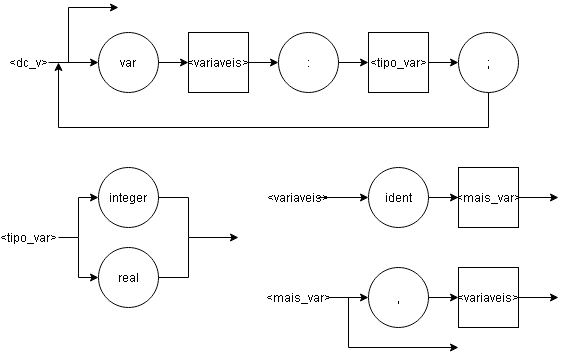
\includegraphics[width=0.5\textwidth]{p1/p1_grafo1.png}
\end{figure}
Podemos substituir o grafo <tipo\_var> em <dc\_v>, e o grafo <mais\_var> em <variaveis>. Com isso reduzimos de quatro grafos para dois.
\begin{figure}[ht!]
    \centering
    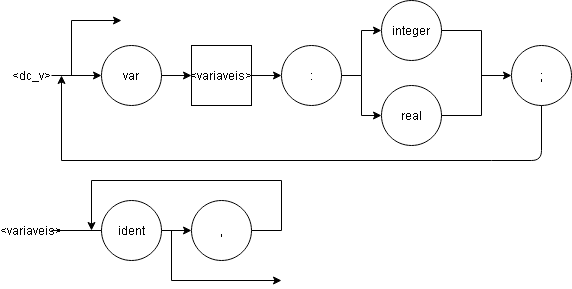
\includegraphics[width=0.5\textwidth]{p1/p1_grafo2.png}
\end{figure}

\subsection{Construa o(s) procedimento(s) recursivo(s) para o analisador sintático destas 4 regras. Crie
também o procedimento principal que inicializa a análise sintática.}
\begin{lstlisting}
procedimento <dc_v>
begin
    se simbolo = var entao
        obter_simbolo
        variaveis
        se simbolo = : entao
            se simbolo = real ou simbolo = integer entao
                obter_simbolo
                se simbolo = ; entao
                    obter_simbolo
                    dc_v
                senao
                    erro
            senao
                erro
        senao
            erro
end

procedimento <variaveis>
begin
    se simbolo = ident entao
        obter_simbolo
        se simbolo = , entao
            variaveis
    senao
        erro
end

procedimento ASD
begin
    obter_simbolo
    dc_v
    se terminou_cadeia entao
        sucesso
    senao
        erro
end
\end{lstlisting}

\newpage
\section{Considere a gramática abaixo com as seguintes 3 regras. Considerando uma análise preditiva não recursiva, monte a tabela sintática completa, com tratamento de erros.}



\begin{lstlisting}
<S> ::= 0<X>1 | cc<C>
<X> ::= x<X> | $\lambda$
<C> ::= c
\end{lstlisting}


Primeiramente vamos definir os conjuntos Primeiro e Seguidor de cada símbolo não terminal:


\begin{lstlisting}
$P(S) = \{0, c\}$
$P(X) = \{x, \lambda\}$
$P(C) = \{c\}$
\end{lstlisting} 
 
 
 
\begin{lstlisting} 
$S(S) = \{\lambda\}$
$S(X) = \{1\}$
$S(C) = \{\lambda\}$
\end{lstlisting} 


Agora criaremos a tabela sintática utilizando as regras da gramática:
\\


\begin{center}
\begin{tabular}{ |c|m{2cm}|m{2cm}|m{2cm}|m{2cm}|m{2cm}|m{2cm}| } 
 \hline
 & $0$ & $1$ & $c$ & $x$ & $\lambda$\\
 \hline
 $S$ & $S \rightarrow 0X1$ & $ $ & $S \rightarrow ccC$ & $ $ & $ $ \\
 \hline
 $X$ & $ $ & $ $ & $ $ & $X \rightarrow xX$ & $X \rightarrow \lambda$\\
 \hline
 $C$ & $ $ & $ $ & $C \rightarrow c$ & $ $ & $ $\\
 \hline
\end{tabular}
\end{center} 


Note que o símbolo $X$ pode se apagar (utilizando a segunda regra da gramática). Dessa forma, precisamos utilizar os elementos do conjunto seguidor $S(X)$ para indicar na tabela como obter o $1$:
\\


\begin{center}
\begin{tabular}{ |c|m{2cm}|m{2cm}|m{2cm}|m{2cm}|m{2cm}|m{2cm}| } 
 \hline
 & $0$ & $1$ & $c$ & $x$ & $\lambda$\\
 \hline
 $S$ & $S \rightarrow 0X1$ & $ $ & $S \rightarrow ccC$ & $ $ & $ $ \\
 \hline
 $X$ & $ $ & $\color{blue}{X \rightarrow \lambda}$ & $ $ & $X \rightarrow xX$ & $X \rightarrow \lambda$\\
 \hline
 $C$ & $ $ & $ $ & $C \rightarrow c$ & $ $ & $ $\\
 \hline
\end{tabular}
\end{center} 


Para os demais cenários, será necessário tratamento de erro.

Para reagir a uma entrada que se encontra no conjunto seguidor de um símbolo não-terminal, a tratativa de erro será de desempilhá-lo.
\\


\begin{center}
\begin{tabular}{ |c|m{2cm}|m{2cm}|m{2cm}|m{2cm}|m{2cm}|m{2cm}| } 
 \hline
 & $0$ & $1$ & $c$ & $x$ & $\lambda$\\
 \hline
 $S$ & $S \rightarrow 0X1$ & $ $ & $S \rightarrow ccC$ & $ $ & $\color{red}{\text{Desempilhar}}$ \\
 \hline
 $X$ & $ $ & $X \rightarrow \lambda$ & $ $ & $X \rightarrow xX$ & $X \rightarrow \lambda$\\
 \hline
 $C$ & $ $ & $ $ & $C \rightarrow c$ & $ $ & $\color{red}{\text{Desempilhar}}$\\
 \hline
\end{tabular}
\end{center} 


Para os outros, precisaremos usar a função de erro de forma a encontrar um ponto de sincronização.

O primeiro grau de sincronização será utilizando o conjunto primeiro de um símbolo não-terminal: São consumidos caracteres de entrada até que encontrado algum símbolo terminal (excluindo-se o $\lambda$) que consta no conjunto.

Caso não sejam encontrados, o segundo grau de sincronização é a procura dos símbolos terminais (excluindo-se o $\lambda$) do conjunto seguidor deste símbolo não-terminal.

Dessa forma, a tabela ficará da forma:
\\


\begin{center}
\begin{tabular}{ |c|m{2cm}|m{2cm}|m{2cm}|m{2cm}|m{2cm}|m{2cm}| } 
 \hline
 & $0$ & $1$ & $c$ & $x$ & $\lambda$\\
 \hline
 $S$ & $S \rightarrow 0X1$ & $\color{red}{\text{Erro(\{$0$, $c$\})}}$ & $S \rightarrow ccC$ & $\color{red}{\text{Erro(\{$0$, $c$\})}}$ & $\color{red}{\text{Desempilhar}}$ \\
 \hline
 $X$ & $\color{red}{\text{Erro(\{$x$\} + \{$1$\})}}$ & $X \rightarrow \lambda$ & $\color{red}{\text{Erro(\{$x$\} + \{$1$\})}}$ & $X \rightarrow xX$ & $X \rightarrow \lambda$\\
 \hline
 $C$ & $\color{red}{\text{Erro(\{$c$\})}}$ & $\color{red}{\text{Erro(\{$c$\})}}$ & $C \rightarrow c$ & $\color{red}{\text{Erro(\{$c$\})}}$ & $\color{red}{\text{Desempilhar}}$\\
 \hline
\end{tabular}
\end{center}

\end{document}
